\chapter{D\'etection et analyse des mots-cl\'es}
\label{chap:keywords}
Afin d'identifier les mots-cl\'es pr\'esents dans le texte d'un \'etudiant et les comparer avec ceux fournis par l'enseignant, nous avons d\'ecid\'e d'utiliser la racine de chaque mot.
Ce faisant, nous pouvons identifier les mots-cl\'es, peu importe l'accord ou le temps de verbe.
Deux techniques de recherche de racine d'un mot ont \'et\'e examin\'ees: la lemmatisation et la racination (\textit{stemming}).

Lors du choix de la technique utilis\'ee pour la d\'etection et l'analyse des mots-cl\'es, nous avons pris en consid\'eration les contraintes suivantes:
\begin{enumerate}
  \item Le but du projet n'\'etant pas de faire de l'analyse linguistique, une biblioth\`eque devra \^etre utilis\'ee si possible;
  \item La biblioth\`eque doit \^etre \'ecrite en PHP, langage utilis\'e par Moodle, afin de faciliter l'installation du module d'extension d\'evelopp\'e;
  \item La biblioth\`eque doit permettre de trouver la racine des mots en fran\c{c}ais, en anglais, et dans d'autres langues si possible, et ce afin de permettre l'utilisation du module d'extension \`a travers le monde.
\end{enumerate}

\section{La lemmatisation}
La lemmatisation consiste \`a trouver le lemme de chaque mot.
Le lemme est la forme canonique d'un mot, soit l'infinitif pour un verbe, le masculin singulier pour un adjectif, etc.
Par exemple, le lemme du verbe \og aimerait \fg{} est \og aimer \fg{}.
La  technique de lemmatisation utilise habituellement un dictionnaire qui associe toutes les conjugaisons possibles d'un mot \`a son lemme.
Certaines biblioth\`eques vont m\^eme consid\'erer le contexte afin de trouver le bon lemme.
Les biblioth\`eques de lemmatisation \'ecrites en PHP sont rares.
Lors de nos recherches, aucune de ces biblioth\`eques ne supportait le fran\c{c}ais et l'anglais.

\section{La racination}
La racination consiste \`a trouver la racine (parfois appel\'e radical, ou \emph{stem} en anglais) de chaque mot.
La racine est trouv\'ee par un algorithme en enlevant la fin du mot.
Par exemple, la racine de \og aimerait \fg{} est \og aim \fg{}.
Cette technique ignore la plupart des exceptions.
La racination est moins pr\'ecise que la lemmatisation.
Par exemple, la racine de \og courons \fg{} est la m\^eme que la racine de \og couronnement \fg{}, soit \og couron \fg{}.
La lemmatisation ne fera pas la m\^eme erreur et trouvera les lemmes \og courir \fg{} et \og couronne \fg{}.
En contrepartie, la recherche de la racine sera plus rapide avec un algorithme de racination qu'une recherche dans un dictionnaire de lemmes.

Il existe quelques biblioth\`eques de racination en PHP.
L'une d'entre elles est \texttt{php-stemmer}~\cite{phpstemmer} qui fait la racination en fran\c{c}ais, en anglais, et dans dix autres langues.
Les algorithmes utilis\'es par \texttt{php-stemmer} sont une traduction en PHP des algorithmes \'ecrits en Snowball, un langage d\'evelopp\'e pour la racination.
%
Comme nous avons trouv\'e une biblioth\`eque de racination qui satisfait tous les crit\`eres et aucune biblioth\`eque de lemmatisation n'en fait autant, pour ce projet nous avons d\'ecid\'e d'utiliser \texttt{php-stemmer} pour l'identification des mots-cl\'es.

\section{Snowball}
Snowball est un petit langage de traitement de texte pour la racination des mots.
Une application Snowball peut \^etre compil\'ee en C ou en Java.
Le site web de Snowball donne l'algorithme de racination pour plusieurs langues: anglais, fran\c{c}ais, espagnol, allemand, russe, etc.

Le langage ainsi que l'algorithme pour la langue anglaise ont \'et\'e d\'evelopp\'es par Porter \cite{snowball}.
%
L'origine des algorithmes pour les langues latines, incluant la langue fran\c{c}aise, n'est pas donn\'ee, mais semble venir aussi de Porter et de contributeurs.

Les algorithmes Snowball sont plut\^ot simples comme on peut le voir dans l'exemple de code~\ref{code:snowball-exemple}.
Cet exemple ex\'ecute une \'etape pr\'eliminaire \`a la racination, soit la gestion des voyelles.
Les lettres en majuscules ne sont plus consid\'er\'ees comme des voyelles pour la racination.
L'algorithme au complet est disponible \`a l'adresse suivante: \url{https://raw.githubusercontent.com/snowballstem/snowball/master/algorithms/french.sbl}
\begin{lstfloat}
\begin{lstlisting}[frame=l]
define v 'aeiouy{a^}{a`}{e"}{e'}{e^}{e`}{i"}{i^}{o^}{u^}{u`}'
define prelude as repeat goto (
    (  v [ ('u' ] v <- 'U') or
           ('i' ] v <- 'I') or
           ('y' ] <- 'Y')
    )
    or
    (  ['y'] v <- 'Y' )
    or
    (  'q' ['u'] <- 'U' )
)
\end{lstlisting}
\caption{Exemple de l'algorithme de racination en fran\c{c}ais en Snowball.}
\label{code:snowball-exemple}
\end{lstfloat}

Les algorithmes Snowball sont structur\'es en plusieurs \'etapes.
Ce qui suit explique les grandes lignes de l'algorithme de racination en fran\c{c}ais, algorithme illustr\'e aussi \`a la figure~\ref{snowball-process} sous forme d'un organigramme%
\footnote{Pour plus d'informations, voir \url{http://snowballstem.org/algorithms/french/stemmer.html}.}.

\begin{figure}[h!]
  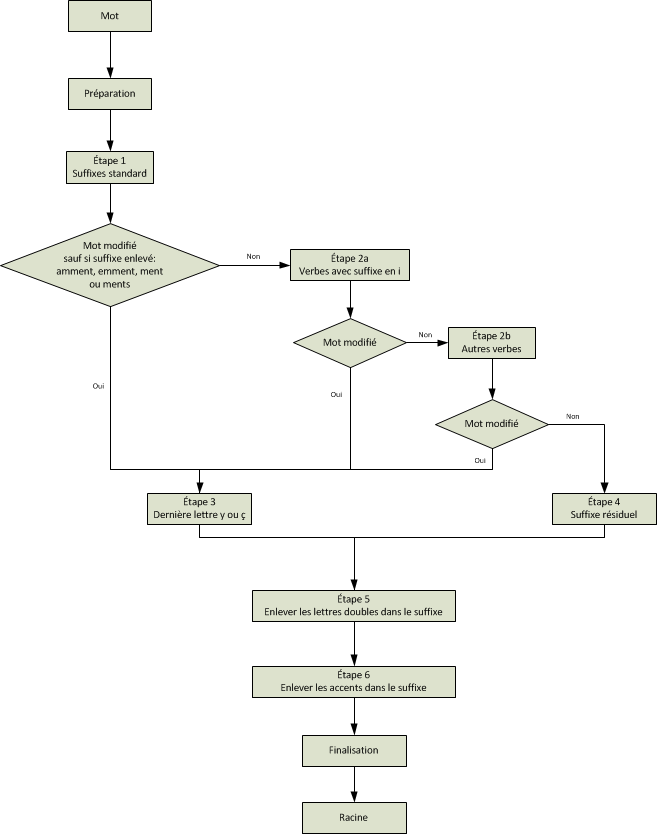
\includegraphics[scale=0.85]{images/snowball.png}
  \caption{Processus de racination Snowball pour la langue fran\c{c}aise.}
  \label{snowball-process}
\end{figure}

\newcommand{\ETAPE}[1]{\item{\emph{#1}}}

\begin{itemize}
\ETAPE{Pr\'eparation}
En se basant sur la position des voyelles, on d\'etermine la section du mot qui pourrait \^etre un suffixe.
\ETAPE{\'Etape 1: Suffixes standards}
Cette \'etape sert \`a trouver la racine des mots, adjectifs, adverbes, etc.
On enl\`eve les suffixes standards (logie, emment, atrice, etc.)
\ETAPE{\'Etape 2: Suffixes de verbes}
Cette \'etape trouve la racine d'un verbe.
Il faut faire cette \'etape seulement si l'\'etape 1 n'a rien chang\'e ou si un des suffixes suivants a \'et\'e trouv\'e: amment, emment, ment et ments.
\begin{itemize}
\ETAPE{\'Etape 2a: Suffixes d\'ebutant par i}
On trouve le suffixe qui d\'ebute par i (\^imes, ie, ira, etc.)
\ETAPE{\'Etape 2b: Autres suffixes de verbes}
On trouve le suffixe de verbe (\'e, era, \^ames, aient, etc.)
\end{itemize}
\ETAPE{\'Etape 3: Derni\`ere lettre}
Si les \'etapes 1 ou 2 ont modifi\'e le mot, faire cette \'etape, sinon passer \`a l'\'etape 4.
Si la derni\`ere lettre est un y, la remplacer par i.
Si c'est un \c{c}, la remplacer par c.
\ETAPE{\'Etape 4: R\'esidu du suffixe}
Il faut faire cette \'etape seulement si les \'etapes~1 \`a 3 n'ont pas modifi\'e le mot.
Cette \'etape sert \`a enlever le pluriel et le f\'eminin des mots proches de leurs racines.
\ETAPE{\'Etape 5: Doublon de la lettre finale}
Les suppressions et remplacements des \'etapes pr\'ec\'edentes peuvent laisser une faute dans la racine du mot.
Cette \'etape sert \`a enlever les lettres doubles de certaines finales de mots (enn, ell, eill, etc.).
\ETAPE{\'Etape 6: Accent final}
Cette \'etape aussi sert \`a nettoyer la racine du mot.
Si un mot se termine par la lettre {\`e ou \'e} suivi d'une ou plusieurs consonnes, enlever l'accent de ce {e}.
\ETAPE{Finalisation}
Finalement, on enl\`eve les majuscules sur les voyelles ajout\'ees durant l'\'etape de pr\'eparation.
\end{itemize}
Au final, on obtient la racine du mot.

Tel que mentionn\'e plus haut, la racination est moins pr\'ecise que la lemmatisaion.
Par exemple les mots \og acceptables \fg{} et \og accept\'e \fg{} ont la m\^eme racine: \og accept \fg{}.
Par contre, le sens des deux mots est tout \`a diff\'erent.


\section{La biblioth\`eque \texttt{php-stemmer} et son utilisation dans notre module}
\label{chap:phpstemmer}
Le fichier \texttt{README.md} du d\'ep\^ot \texttt{git} pour la biblioth\`eque \texttt{php-stemmer} la d\'ecrit comme \'etant \og \textit{[a] PHP5 native implementation of Snowball stemmer} \fg{}~\cite{phpstemmer}.
%
En comparant le code de la biblioth\`eque \texttt{php-stemmer} et les algorithmes Snowball, on peut remarquer que les algorithmes sont les m\^emes.
\texttt{php-stemmer} est donc une traduction PHP des algorithmes Snowball.

La biblioth\`eque \texttt{php-stemmer} nous servira donc \`a trouver la racine de chaque mot-cl\'e, de chaque mot dans la r\'eponse de l'\'etudiant ainsi que dans chaque mot dans la r\'eponse de l'enseignant.
De cette mani\`ere, il sera possible de mettre en \'evidence chaque mot-cl\'e dans la r\'eponse de l'\'etudiant, peu importe l'accord.

Par exemple, supposons que l'enseignant donne \og illumination \fg{} comme mot-cl\'e et l'\'etudiant donne la r\'eponse \og Le pont Jacques-Cartier \`a \'et\'e illumin\'e pour le 375\textsuperscript{e} de la ville de Montr\'eal. \fg{}.
La racine du mot-cl\'e \og illumination \fg{}  est \og illumin \fg{}.
En examinant la racine de chaque mot dans la r\'eponse de l'\'etudiant, on constate que la racine du mot \og illumin\'e \fg{} est aussi \og illumin \fg{}.
Il faut donc mettre en \'evidence le mot \og illumin\'e \fg{} lorsqu'on affiche la r\'eponse au correcteur.
Le module d'extension devra afficher la r\'eponse de l'\'etudiant avec le mot illumin\'e en \'evidence tel qu'illustr\'e dans la phrase suivante: \og Le pont Jacques-Cartier \`a \'et\'e \textbf{\underline{illumin\'e}} pour le 375\textsuperscript{e} de la ville de Montr\'eal. \fg{} 
